\documentclass[MAIN.tex]{subfiles} 
\begin{document} 
	\begin{frame}
		\begin{figure}
\centering
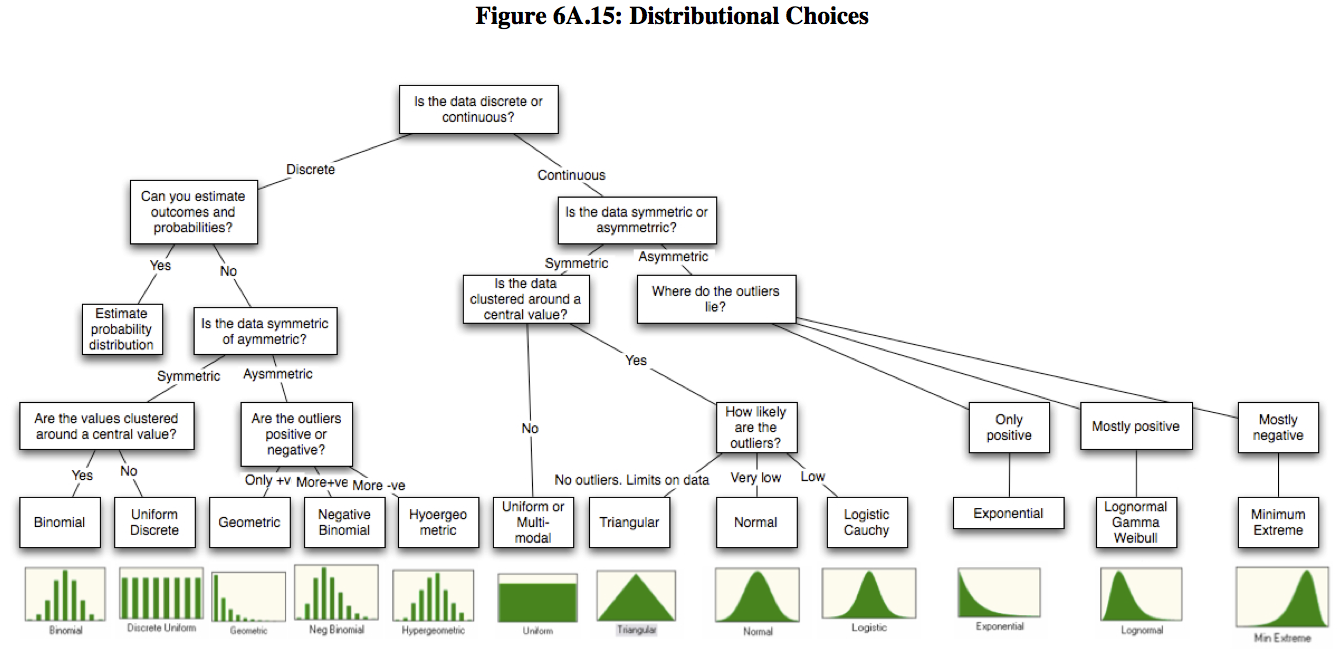
\includegraphics[width=1.05\linewidth]{C:/Users/Kevin/Documents/GitHub/ProbDistributionsWithR/images/flowchart}

\end{figure}

	\end{frame}
	\begin{frame}
		\begin{figure}
\centering
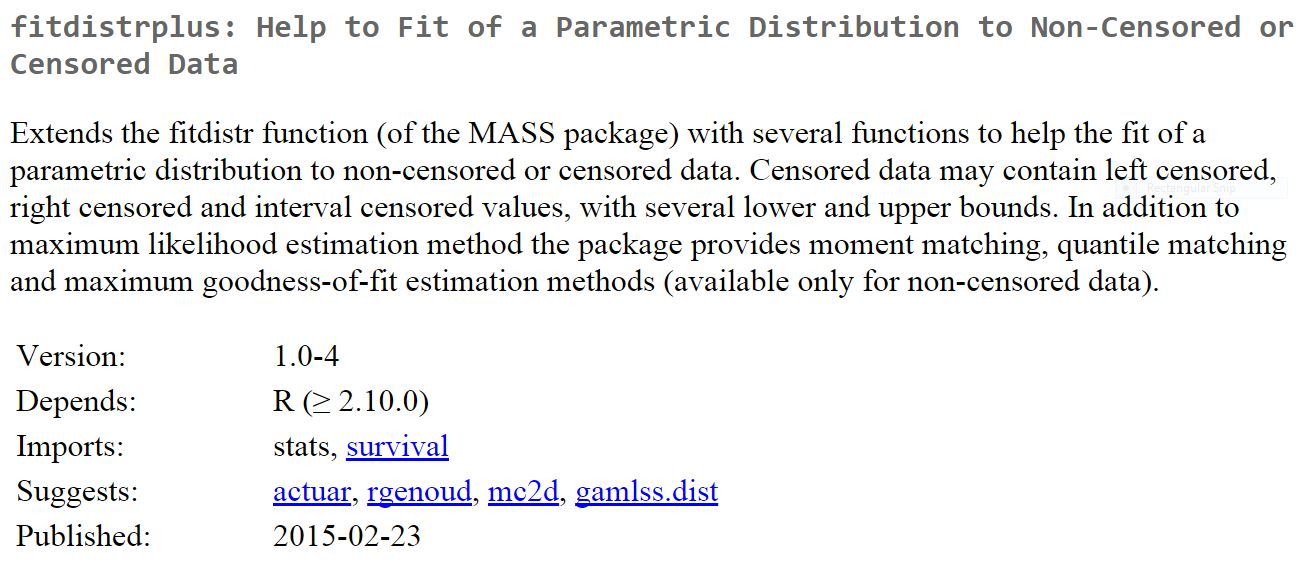
\includegraphics[width=1.05\linewidth]{C:/Users/Kevin/Documents/GitHub/ProbDistributionsWithR/images/fitdistrplus}

\end{figure}

	\end{frame}
	\begin{frame}
		\begin{figure}
\centering
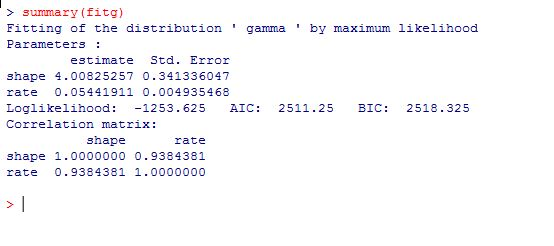
\includegraphics[width=1.05\linewidth]{C:/Users/Kevin/Documents/GitHub/ProbDistributionsWithR/images/fitdistrplus2}
\caption{}
\label{fig:fitdistrplus2}
\end{figure}

	\end{frame}
\end{document}